\chapter{Component Selection and Design}
\justifying
\section[Solar Panels]{Solar Panels}
 TJ Solar Cell 3G30C - Advanced is selected. This cell is a GaInP/GaAs/Ge on Ge substrate triple junction solar cell. The end-of-life version of the 3G30C solar cell offers best EOL-performance
 values. Connected to the EPS via an external bypass diode protection.
 
 Specifications:
 \begin{itemize}
 	\item Average Open Circuit Voltage: 2.7 V
 	\item Maximum Power Point Voltage: 2.41 V
 	\item Average Short Circuit Current: 520.2 mA
 	\item Maximum Power Point Current: 504.4 mA
 \end{itemize}
It has an average efficiency of 29.8\% at 1353 $W/m^{2}$. This solar cell is excellent for space applications. 
\\

Since a CubeSat has six sides and one cell of selected model fits half of a side, a total of 12 cells can be placed.\\ 

Power from a solar panel, P :\\
\hspace*{2cm} $P = P_{i} \times Area \times \eta  \times cos \alpha $ 
\\
 Where, \\
 $P_{i}$ = incident power from sun (1367 W/$m^2$ at Low Earth Orbit)
\\  $\eta$ = conversion efficiency of cell (take 20\% for contingency)
\\  $\alpha$ = angle between normal of cell and incident light (avg: $35^{o} $)\\ \\
Area of solar cell at one face : 0.0032 * 2 = 0.0064 $m^2$\\
\\ \\ Therefore, $P = 1367 W/m^2 \times 0.0064 \times 20  \times cos 35^{o} $ = 1.43 W\\

Assume two faces of CubeSat is lit by sunlight every time except eclipse and total sun time($T_{s}$) is 1 hour (from orbital parameters).
\\ \\ Therefore, total energy produced is, $P \times  T_{s}$ = $(1.43 \times 2) \times 1$ = 2.86 Wh
\\ \\ \textbf{Of all modes specified in power budget, nominal mode at sun phase with transmission and payload ON consumes the most energy (1.016 Wh), and most energy consumed at eclipse phase is 0.769 Wh. This add upto 1.785 Wh, which is the worst case energy demand. This can be compensated by the designed solar panel configuration.}
\\
Solar panels are connected in such a way that each side has two cells connected in series.The maximum voltage developed per side is 4.4 V and the maximum current that can be generated per side at peak power point is 0.5 A.
Panels on opposite sides are connected in parallel.


\section[MPPT Circuit]{Maximum Power Point Tracking Circuit}

Maximum Power Point Tracking (MPPT) is a technique used in photovoltaic (PV) systems to optimize the power output of the PV panel. The goal of MPPT is to ensure that the PV panel operates at its maximum power point (MPP), which is the point on the current-voltage (I-V) curve of the panel where the panel can produce the maximum amount of power.
\\ \\
As each solar panel has different temperatures and incident radiance angles, the
Maximum Power Point (MPP) is also different. So each solar panel has a MPPT
converter to assure that the maximum power available at the solar panels is
transferred independently from their working power points. Since the peak power
point cannot be accurately predicted, many different algorithms exist for finding
the best approximation. MPPT controllers use different algorithms such as {\bf Perturb and Observe (P\&O), Incremental Conductance, and Fuzzy Logic} to track the MPP. These algorithms operate by incrementally changing the load impedance of the panel and measuring the corresponding change in voltage and current until the MPP is reached.
\\ \\
The SPV1040 was chosen as the MPPT IC. It is a boost converter with duty ratio controlled by Perturb and Observe MPPT algorithm. The perturb and observe algorithm is based on monitoring either the voltage or the current supplied by the DC power source unit so that the PWM signal duty cycle is increased or decreased step-by-step according to the input power trend. This chip has inbuilt over-current protection and a cutoff mechanism if the solar panel connection is reverse-inserted to prevent damage to the IC and the external circuit.
\\ \\
The MPPT IC can only handle 1.8 A of input current. Also, the input voltage of each MPPT must be much less than the desired output voltage for them to function properly. Depending on the configuration, the number of MPPT ICs was calculated to be 6.
\\ \\
Each side of cubesat consists of two 2.4 V cells, each cells giving a maximum current output of 500 mA for each MPPT, which is well below the maximum current the IC can handle. One cell from opposite sides are connected to its own MPPT, which is set to boost to 5.2 V. The MPPTs are then connected in parallel.
\\ \\
Connecting multiple regulators in parallel can sometimes cause problems if one source is outputting a slightly smaller or larger voltage than the others. In most cases, the use of ballast resistors solves this problem. The footprint for a 25 mohm ballast resistor will be chosen to be included in series with the output of each MPPT.\\



Specifications of  SPV1040 [7]:
	\begin{itemize}
	\item Input Voltage: 0.3 - 5.5 V
	\item Output Voltage: 5 V
	\item Switching Frequency: 100 kHz
%	\item Inbuilt over-current, temperature protection
	\item Efficiency: 95\%
\end{itemize}
The MPPT circuit schematic is shown below:
 	\begin{figure}[h]
	\centering
	\includegraphics[width=\columnwidth]{IMGS/MpptDemoBoard.pdf}
	\caption{MPPT circuit with SPV1040}
	\label{fig:mpptsch}
\end{figure}
\subsection{PCB Layout}
The PCB was designed in KiCad EDA software
The MPPT PCB layout is shown below:
\begin{figure}[H]
	\centering
	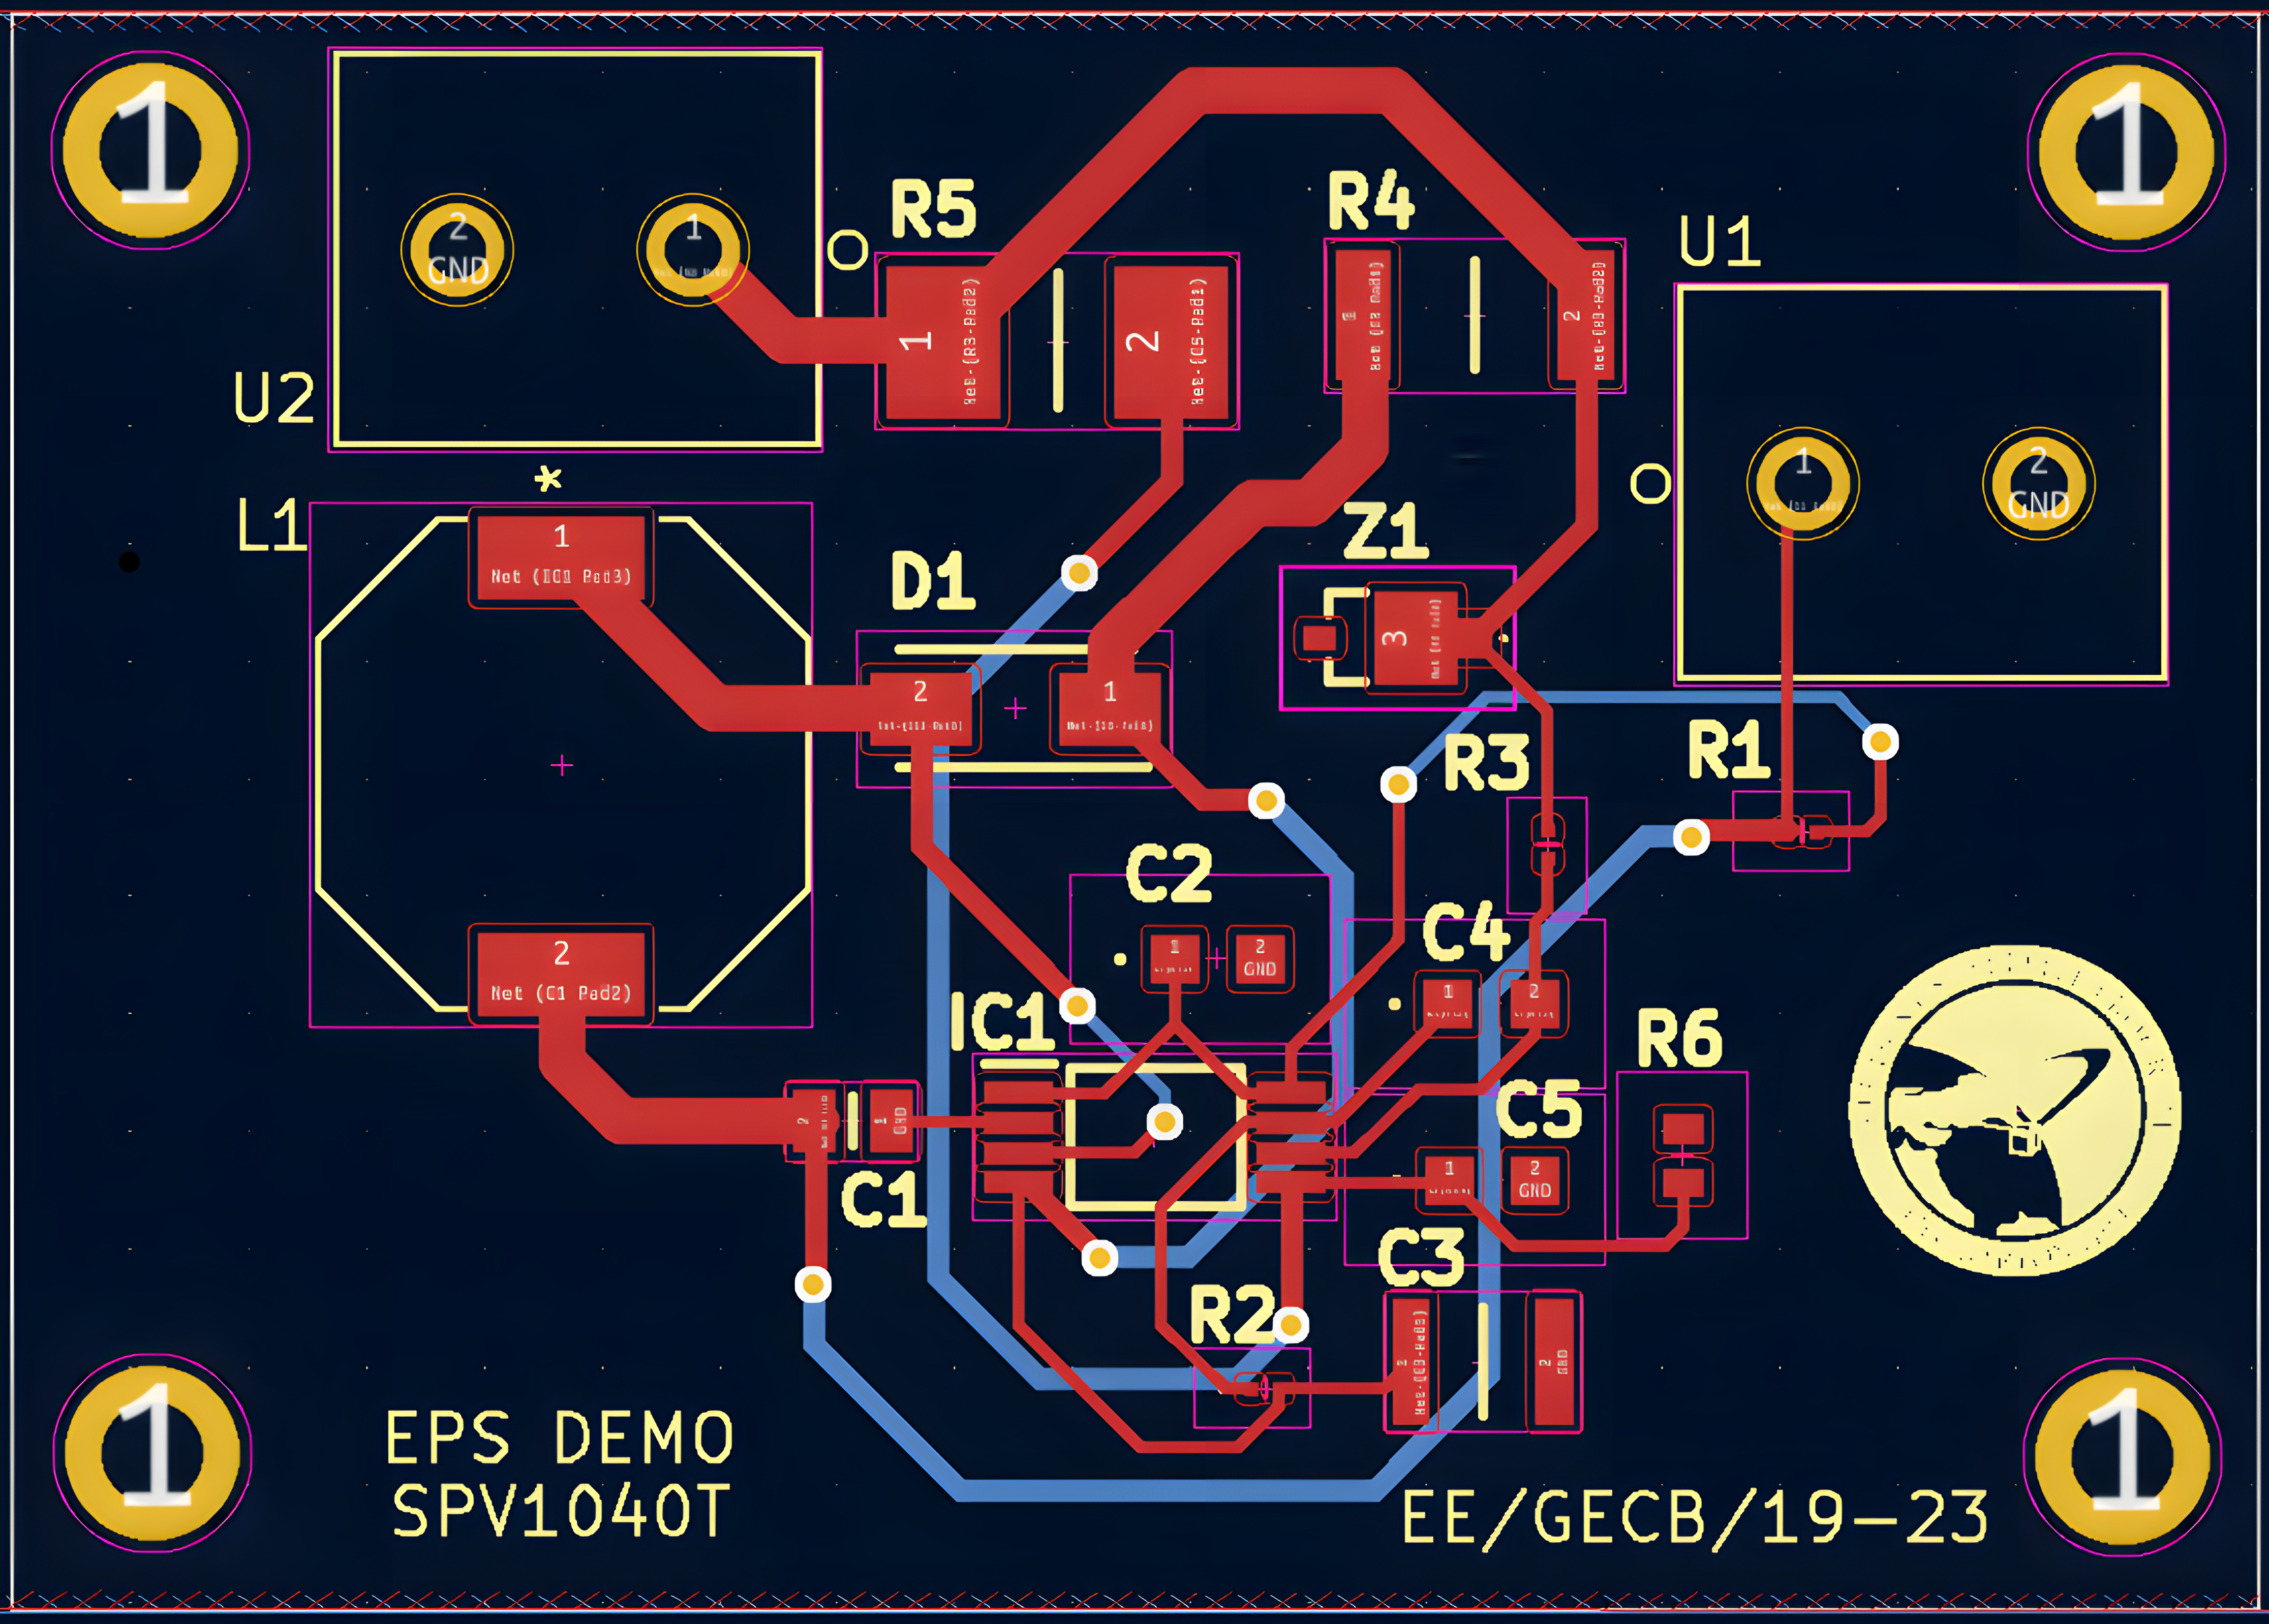
\includegraphics[width=0.7\columnwidth]{IMGS/MpptDemopcb.jpg}
	\caption{MPPT PCB Design}
	\label{fig:mpptpcb}
\end{figure}

The 3D model of the MPPT PCB is shown below:
\begin{figure}[H]
	\centering
	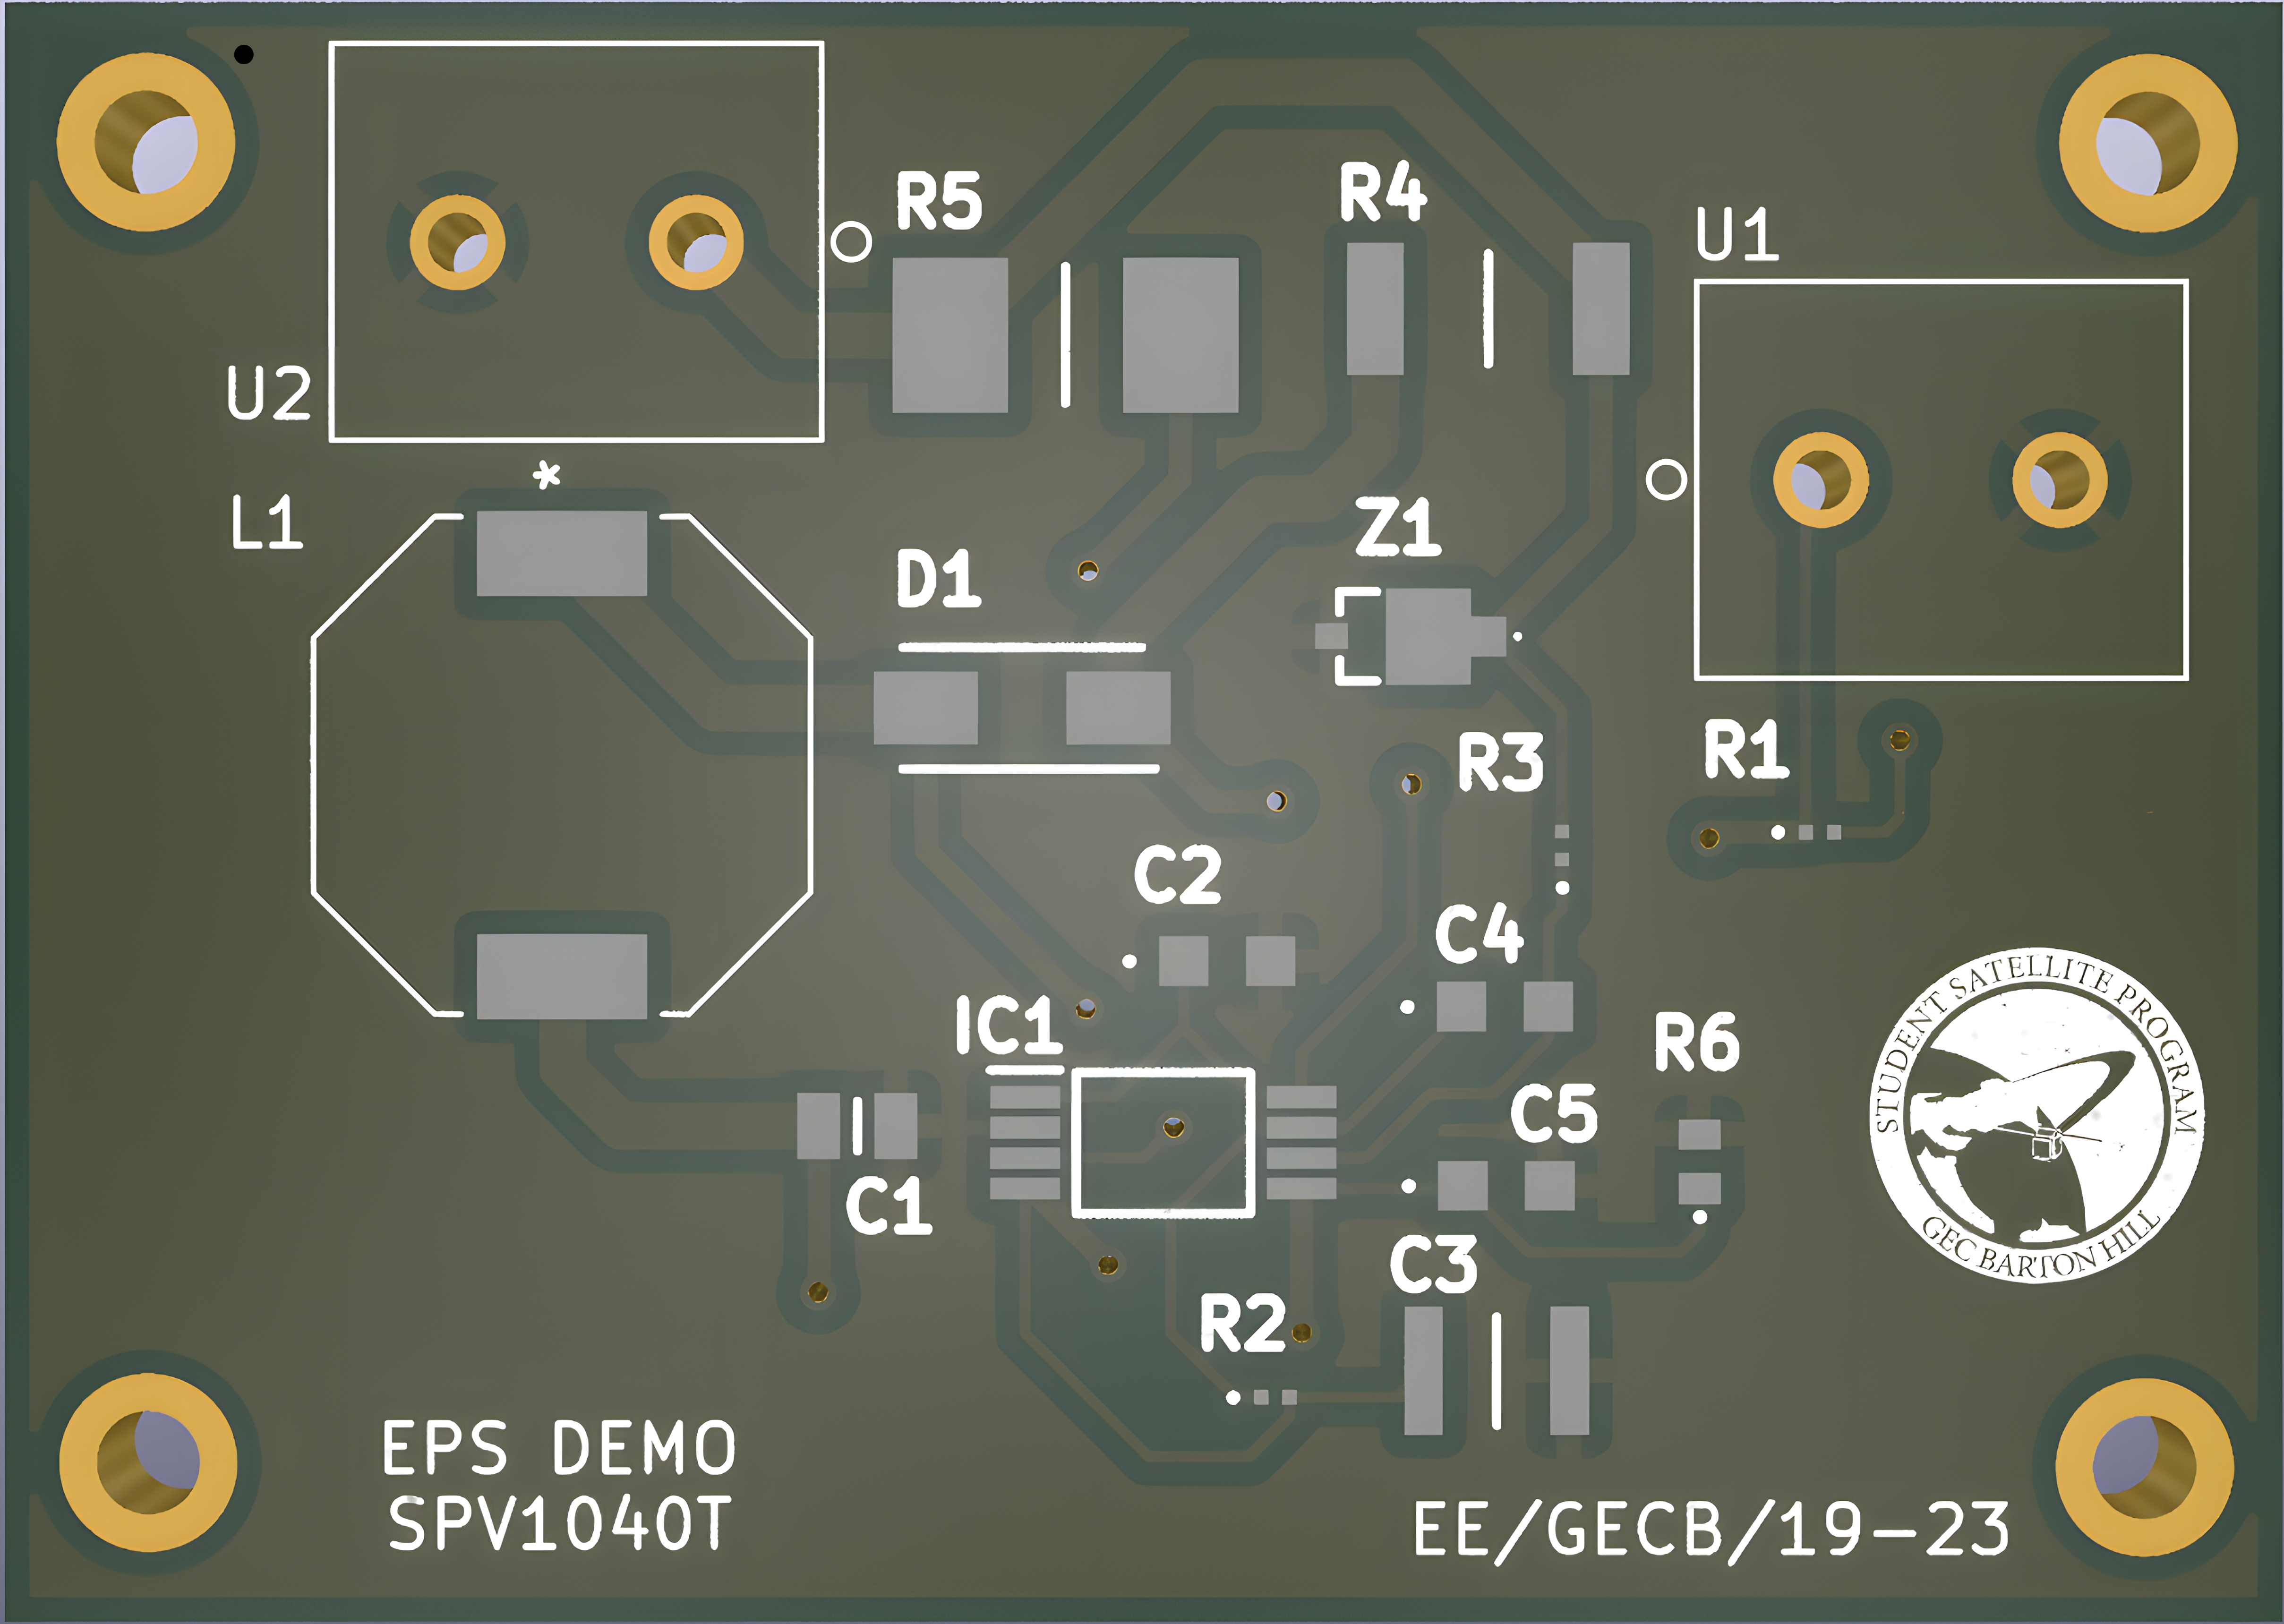
\includegraphics[width=0.7\columnwidth]{IMGS/MpptDemo3d.jpg}
	\caption{MPPT 3D}
	\label{fig:mppt3d}
\end{figure}





\section[Battery]{Battery}
The most popular types of batteries use the following materials: Nickel Cadmium
(NiCd), Nickel Metal Hydride (NiMH), Nickel Hydrogen (NiH2), Lithium Ion
(Li-Ion) and Lithium Polymer (Li-Po). The Li-Po and Li-Ion became the standard use in space technology due to their
high energy density (Upto 200 Wh / kg on Li-Po and upto 250 Wh / kg on Li-Ion) and also due to
the number of charging cycles being as high as the NiMH, whilst presenting higher
operating temperatures. 
\subsection{Battery Selection}
According to solar power calculations, the solar panel can produce 2.86 Wh of energy in a single orbit, of which 1.016 Wh will be used up in sun phase in worst case ($E_{max}$). So there will be atleast 1.844 Wh of energy left to charge the battery.\\
In power budget, the most amount of energy required during eclipse phase is 0.769 Wh.\\ \\
Assign 50\% contingency, the battery needs energy of 1.1535 Wh for charging, to use in worst case eclipse mode. This energy corresponds to 30\% of total battery capacity (End Of Life capacity of battery).\\ \\
So, we need a battery with Beginning Of Life capacity of 3.845 Wh.\\ \\
\hspace*{5cm}Required Ah of battery = $\frac{Estimated\;\; Wh}{Battery\;\; Voltage}$
\\ \\ \hspace*{5cm}So, required Ah = $\frac{3.845 Wh}{3.6 V}$ = 1.068 Ah\\


Considered options are Samsung 18650 and Panasonic 18650 Li-ion cells. Samsung 18650 has 2500 mAh capacity, 3.6 V and a capacity loss of 60\% after 250 charging cycles ($N_{in}$=250). Panasonic 18650 has 3350 mAh capacity, 3.6 V and a capacity loss of 60\% after 300 charging cycles ($N_{in}$=300).\\ \\
for a CubeSat mission of 3 months, required battery cycles will be around 1460 cycles (since each day, CubeSat goes through 16 sun phase).\\ \\
Total no. of cycles a cell can provide = $N_{T}$\\ \\
\hspace*{3cm} $N_{T} = \frac{N_{in} \times C_{B}}{C_{exp}}$
\\ 
Where,\\
$N_{in}$ = initial number of cycles a battery can provide)
\\ $C_{B}$ = Capacity of the battery
\\ $C_{exp}$ = Capacity expected to use\\
%Capacity expected to use = $C_{exp}$\\ \\
\hspace*{3cm} $C_{exp} = \frac{E_{max}}{V_{B}}$
\\ Where,\\
 $E_{max}$ = Maximum energy consumed in a phase with 50\% contingency
\\ $V_{B}$ = Battery voltage\\ \\
Therefore, $C_{exp} = \frac{1.524}{3.6V}$ = 450 mAh \\ \\
Total no. of cycles Samsung 18650 can provide =$\frac{250 \times 2500}{450}$ = 1388 cycles\\ \\
Total no. of cycles Panasonic 18650 can provide =$\frac{300 \times 3350}{450}$ = 2200 cycles\\ 

\textbf{Therefore, Panasonic 18650 is selected, as it can compensate the charging cycle requirements.}
Specifications of Panasonic NCR 18650 GA Li-Ion cell:
\begin{itemize}
	\item Voltage: 3.7 V - 4.2 V
	\item Capacity: 3500 mAh
	\item Can withstand 2200 charge-discharge cycles
	\item 1800 cycles till capacity reduces to 60\%
\end{itemize}
\section[Battery Charger]{Battery Charger}
 The battery also needs a charger to regulate its current and voltage while charging.
 BQ25302, a synchronous Buck Battery Charger IC was selected and connected in external power path mode as given in the data-sheet. The BQ25302 is a highly-integrated standalone
 switch-mode battery charger for single cell Li-Ion batteries. It supports input voltage in the range of 4.1 V to 6.2 V and maximum charging current of 2 A. It has a very low quiescent current of 200 nA to conserve battery during idle.
 It detects the charge
 voltage setting at startup and charges the battery in four phases: battery short, pre - conditioning, constant
 current, and constant voltage. \\
 
 The charger incorporates various safety features for battery charging and system
 operations, including battery temperature monitoring based on negative temperature coefficient (NTC)
 thermistor, charge safety timer, input over-voltage and over-current protections, as well as battery over-voltage
 protection. Thermal regulation regulates charge current to limit die temperature during
 high power operation or high ambient temperature conditions.
 \\
 
 The STAT pin output reports charging status and fault conditions. It is connected to REGN via a current
 limiting resistor and LED. Blinking LED indicated a fault condition.\\
 
 The battery charge voltage setting is done by the VSET pin. As the Panasonic NCR 18650 GA Li-Ion cell with a charge voltage of 4.2 V was selected the VSET pin was shorted to ground to set the battery charge voltage to 4.2 V.
 
 
 To preserve battery life, the charging current has to be limited. The charging current provided to the battery by BQ25302 IC can be limited by adjusting the resistor value at the ICHG pin according to the equation below:
 \begin{equation}
 	I_{CHG} (A) = K_{ICHG} (A.\ohm) / R_{ICHG} (\ohm)
 	\label{eq:6.1}
 \end{equation}
 Where,
 \begin{itemize}
 	\item $I_{CHG}$ is the charging current
 	\item $K_{ICHG}$ is the charge current ratio.  The $K_{ICHG}$ vs.
 	$I_{CHG}$ typical characteristic curve is shown in fig. \ref{fig:kichg}
 	\item $R_{ICHG}$ is the resistor value at the ICHG pin 
 \end{itemize}
 
  \begin{center}
 	\begin{figure}[h]
 		\centering
 		\includegraphics[width=0.7\columnwidth]{kich.png}
 		\caption[$K_{ICHG}$ vs. $I_{CHG}$ characteristics]{\centering $K_{ICHG}$ vs. $I_{CHG}$ characteristics (Source: [8])}
 		\label{fig:kichg}
 	\end{figure}
 \end{center}
 From the fig. \ref{fig:kichg}, it is clear that the value of $K_{ICHG}$ should be 40200 to limit the charging current near to 1.2 A. Thus, from equation \ref{eq:6.1} the calculated value of resistance at the ICHG pin is 33.5 k\ohm.
 \\
 
 The IC is connected in an external power path configuration by connecting an external PFET for the battery. The PFET turns on when there is no external supply available from the solar panels and the system has to be powered by the battery. It is also useful if the system has to be powered ON when the battery is over-discharged or dead. 
 
 
 Specifications and Operating Conditions of BQ25302 [8]:
\begin{itemize}
 	\item Input Voltage: Upto 5 V
 	\item Output Voltage: Upto 4.2 V
 	\item Switching Frequency: 1.2 MHz
 	\item Output Current: Limited to 1.2 A by connecting a 33.5k resistor at ICHG pin 
 	\item Efficiency: 94.3\% at 1A from 5 V input 
 	\item Thermistor: Semitec 103AT-2 (10\si{\kilo\ohm})
 	\item Charging Temperature: Limited between 0 - 45 $^{o}C$
 \end{itemize}

The Battery Charger circuit schematic is shown below:
\begin{figure}[H]
	\centering
	\includegraphics[width=\columnwidth]{IMGS/charg.pdf}
	\caption{Schematic of Battery Charger circuit with BQ25302}
	\label{fig:battch}
\end{figure}

  \begin{figure}[H]
	\centering
	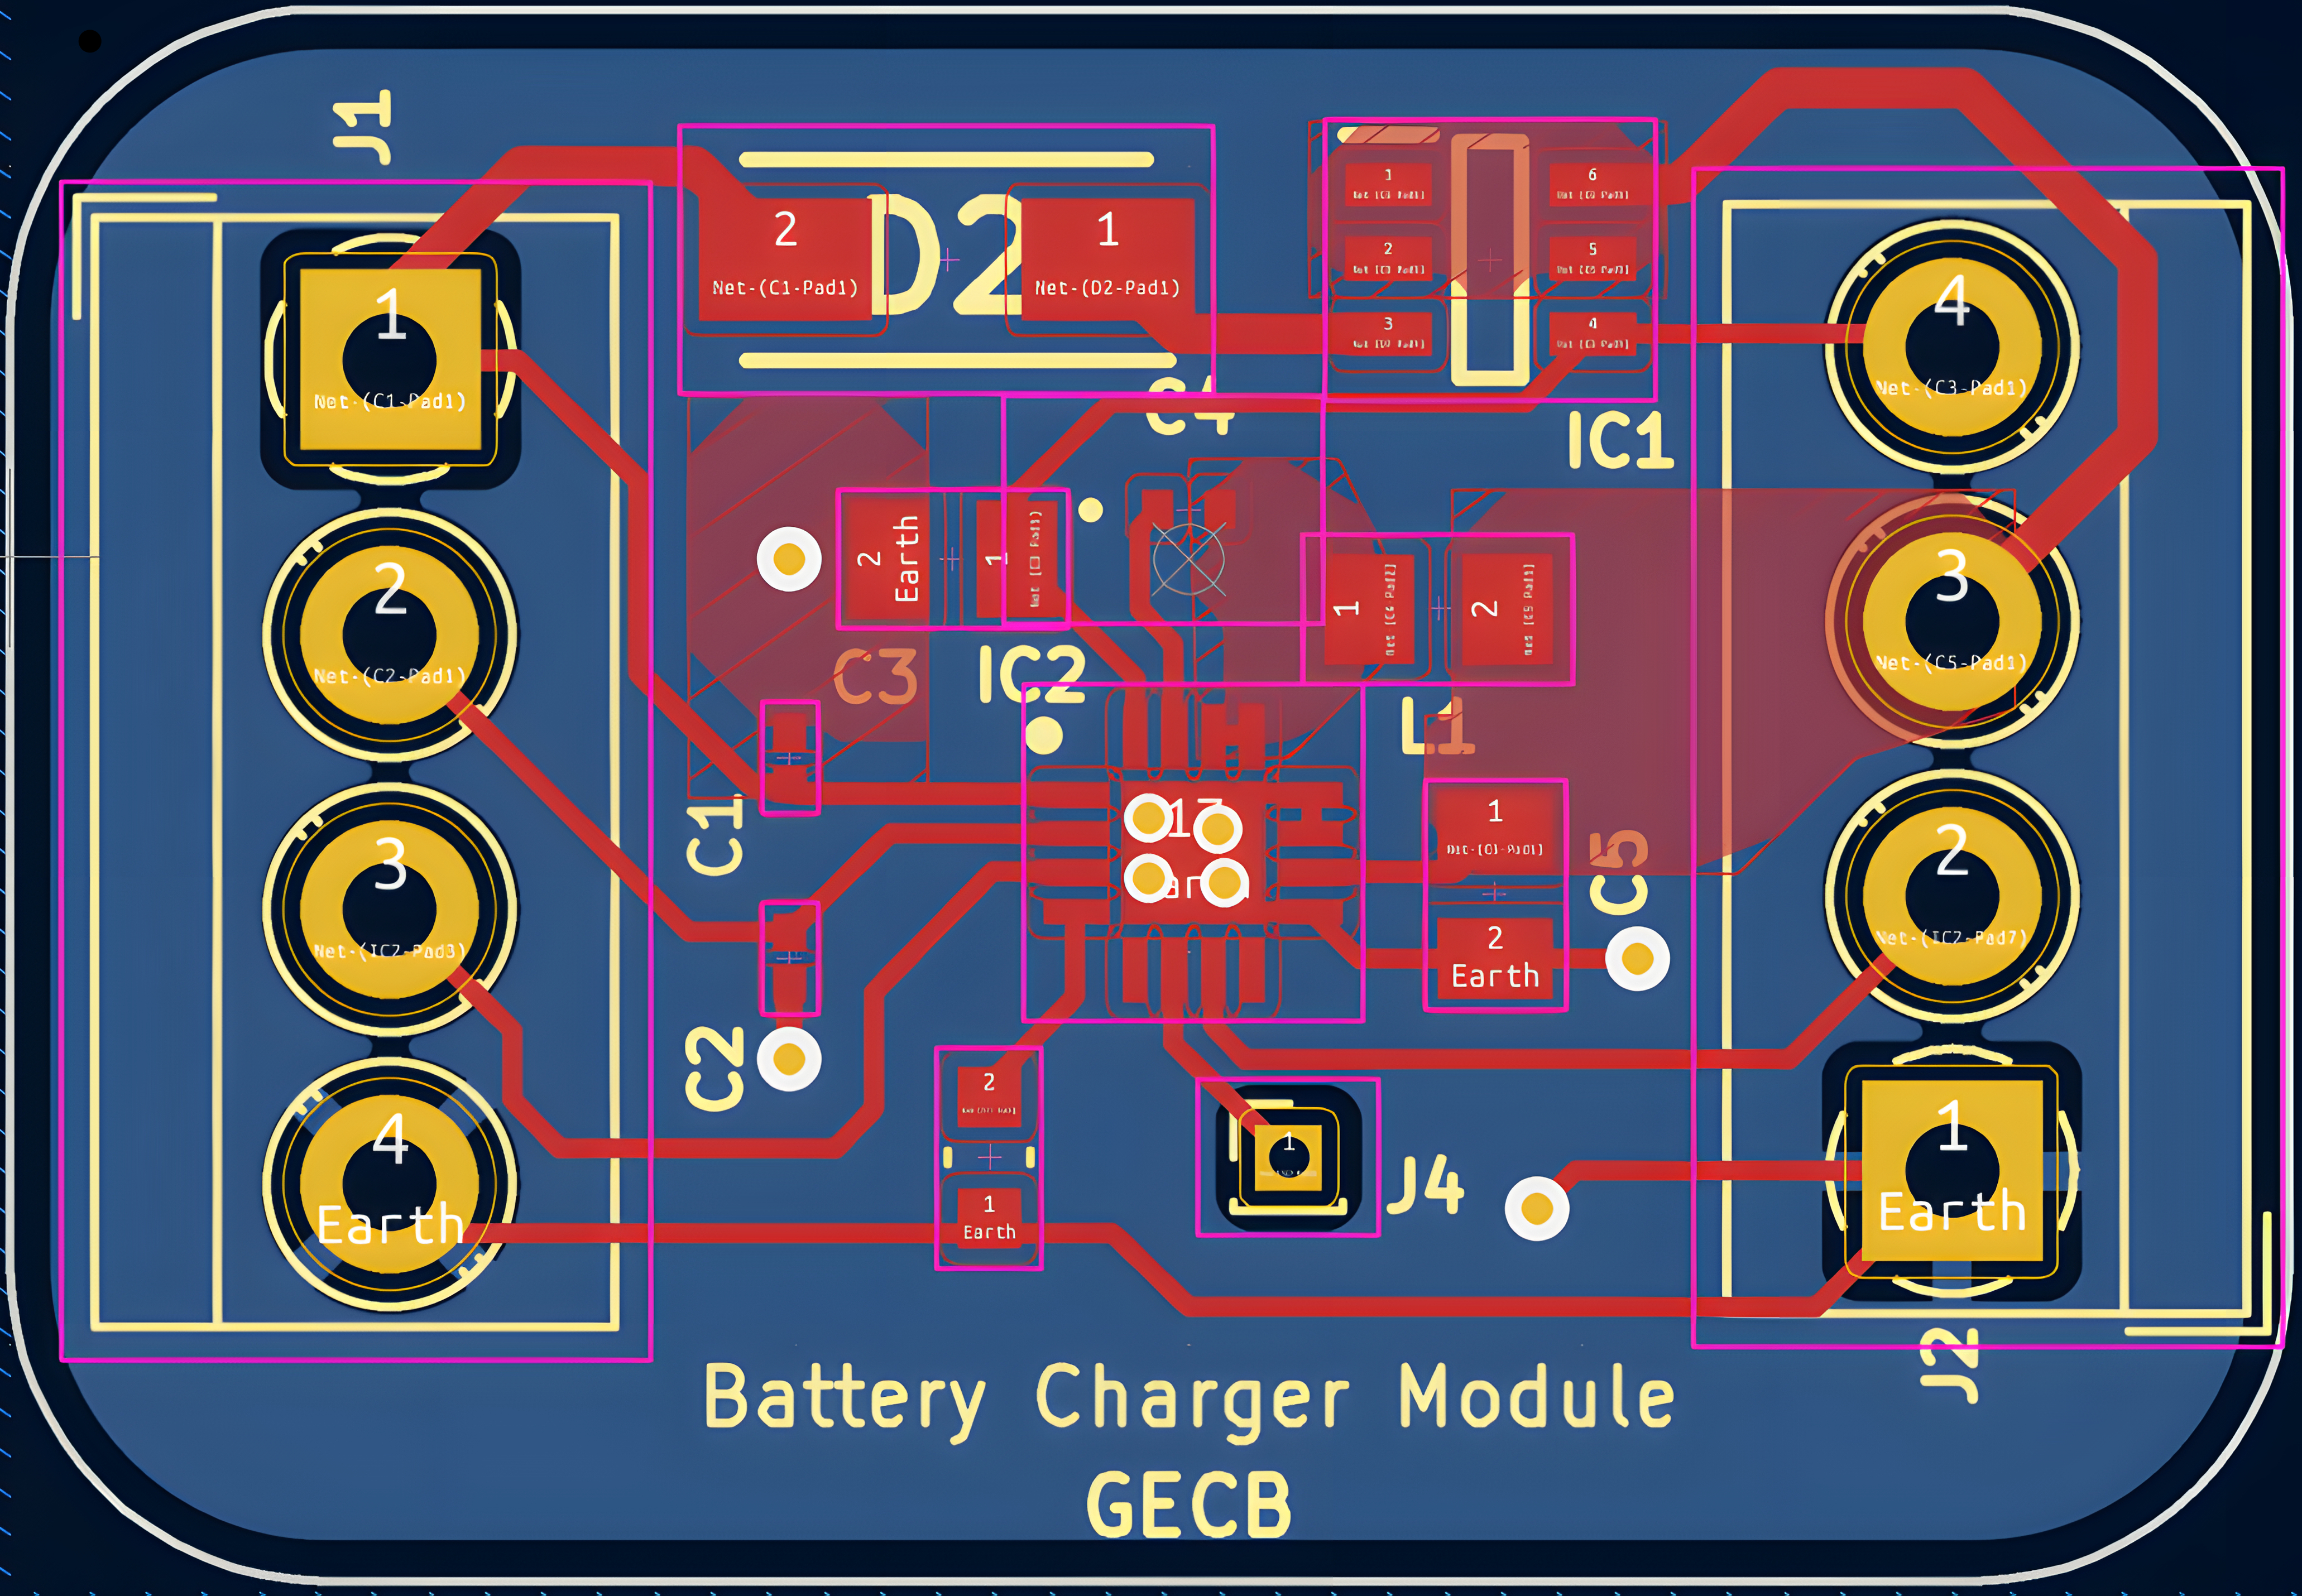
\includegraphics[width=0.6\columnwidth]{IMGS/charg pcb.jpg}
	\caption{\centering Battery Charger circuit PCB - All Copper Layers only}
	\label{fig:chargpcb}
\end{figure}
\begin{figure}[H]
	\centering	\includegraphics[width=0.7\columnwidth]{IMGS/charg 3d.png}
	\caption{\centering Battery Charger circuit PCB - 3D Model}
	\label{fig:chargpcb3d}
\end{figure}

\pagebreak \justifying








\section[Switching Regulators]{Buck and Boost Converters}
The power conditioning is associated with regulating the voltage to accommodate
for the charging voltage and the voltages of the satellite's subsystems. In most
subsystems, the need for a specific voltage requires a regulation of either a step-up
or a step-down of the supplied voltage. It can be done by buck
convertor(step-down) and boost converter(step-up).\\
TPS62203 was selected as the buck converter to provide step down voltage of the DC bus to supply the 3.3 V loads. It is a high-efficiency synchronous step-down converter with up to 95\% efficiency. It operates with a 1MHz fixed frequency (PWM) at moderate loads to heavy load currents and operates with pulse
frequency modulation (PFM) at light load currents.\\

It has a shutdown quiescent current of typically 0.1 {$\mu$}A

 Specifications and Operating Conditions of TPS62203[9]:
\begin{itemize}
	\item Input Voltage: 3.6 - 5 V
	\item Output Voltage:  3.3 V
	\item Switching Frequency: 1 MHz
	\item Output Current: 300 mA (max.)
\end{itemize}


 LTC3426 was selected as the boost converter to provide step up voltage of the DC bus to supply the 5V loads. It has an internal 2 A MOSFET as the switch.\\
 
  Specifications and Operating Conditions of LTC3426[10]:
 \begin{itemize}
 	\item Input Voltage: 3.6 - 5 V
 	\item Output Voltage: 5 V
 	\item Switching Frequency: 1.2 MHz
 	\item Output Current: 500 mA (max.)
 \end{itemize}
All convertors operate in continuous conduction mode.\\

The Buck and Boost Converter circuit schematic is shown below:
\begin{figure}[ht]
	\centering
	\includegraphics[width=\columnwidth]{1.pdf}
	\caption{LTC3426 as boost IC and TPS62203 as buck IC}
	\label{fig:bubo}
\end{figure}



\section[Protection Circuits]{Protection and Measurement Circuits}


LTC4361-2 is selected as the over voltage and over current protection IC. It control an external N-channel MOSFET as a switch to cut the path of current if there is an event of over current or voltage. Manual control of the MOSFET is also possible which may be useful to turn off power to buses by the micro-controller as per different modes of operation of the CubeSat.
\\

 Voltage and current passing through each bus and subsystems are continuously monitored by sensors and this information is fed to the micro-controller. These measurements help in estimation of load requirement of subsystems and also help in triggering of protection circuits if a subsystem needs to be turned off in case of an occurrence of a fault. 
 \\
 
 LTC2990 was chosen as the voltage  and current monitor. It can measure the voltage of four external channels and it's supply voltage ($V_{cc}$) simultaneously. It has a 14 bit ADC for measurement. The LTC2990 has the ability to perform 14-bit current measurements with the addition of a current sense resistor. The measurements are passed on to the micro-controller through the two wire I2C interface.
 \begin{center}
 \begin{figure}[h]
 	\centering
 	\includegraphics[width=\columnwidth]{IMGS/1.pdf}
 	\caption{\centering Schematic of Buck and Boost circuit with Protection and Voltage and Current Measurement ICs}
 	\label{fig:bubo2}
 \end{figure}
\end{center}
The screw terminals are used to connect to the power inputs and outputs of the PCB. Pin header connectors are provided for connecting IC control pins to the micro-controller. The pin headers and their functions are given below:
 \begin{itemize}
 	\item EN pin of Buck IC: Setting LOW turns off the buck IC
 	\item SHDN pin of Boost IC: Setting LOW turns off the boost IC
 	\item ON1 pin of IC1 (LTC4361): Setting HIGH turns off the MOSFET (IC2 - SI470DH) of the 3.3 V bus
 	\item ON2 pin of IC4 (LTC4361): Setting HIGH turns off the MOSFET (IC3 - SI470DH) of the 5 V bus
 	\item SCLSDA1 pins: I2C connection to micro-controller relaying measured parameters of 3.3 V bus by U2 (LTC2990) 
 	\item SCLSDA2 pins: I2C connection to micro-controller relaying measured parameters of 5 V bus by U3 (LTC2990) 
 	\item SCLSDA3 pins: I2C connection to micro-controller relaying measured parameters of input bus ($V_{in}$) by U1 (LTC2990)
 \end{itemize}


\subsection{PCB Layout}
 A double layer PCB was designed from the schematic (Ref. Fig. 8.4). The second layer was used as the GROUND plane. The schematic and PCB design was done in KiCad EDA. 
 
  \begin{figure}[h]
 	\centering
 	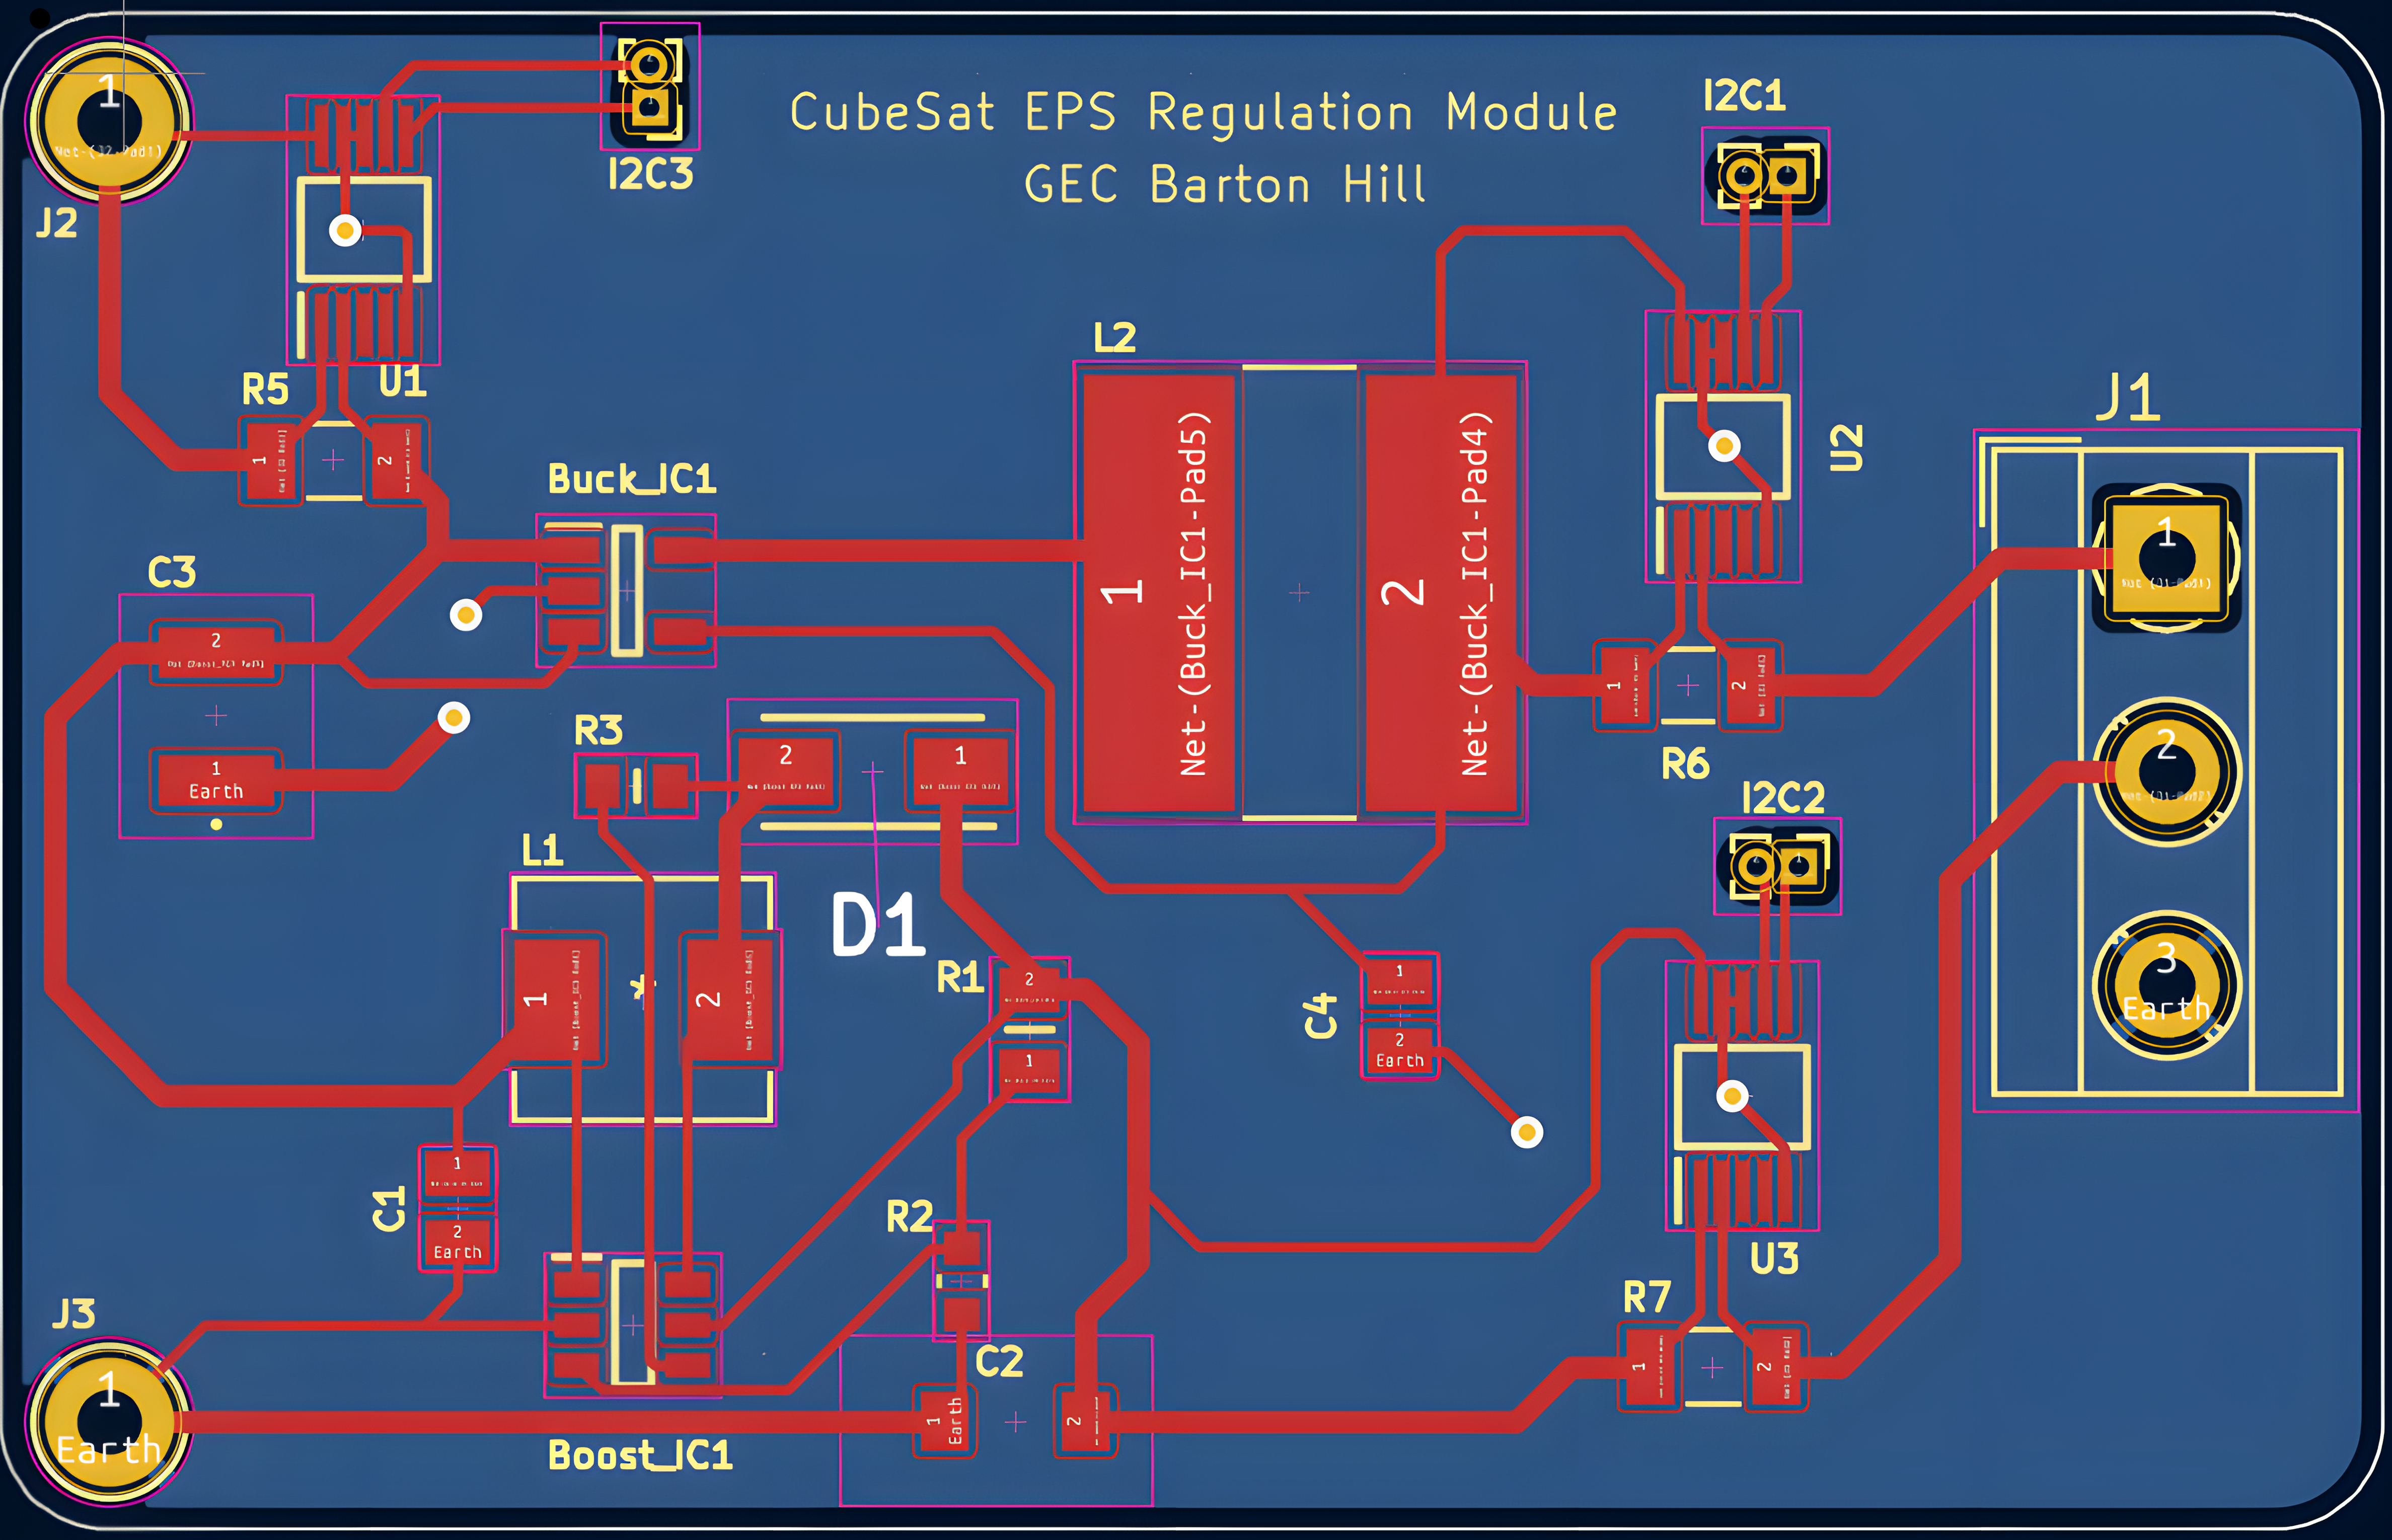
\includegraphics[width=0.6\columnwidth]{IMGS/1 pcb.jpg}
 	\caption{\centering Buck and Boost circuit PCB - All Copper Layers only}
 	\label{fig:bubopcb}
 \end{figure}
 
   \begin{figure}[H]
 	\centering
 	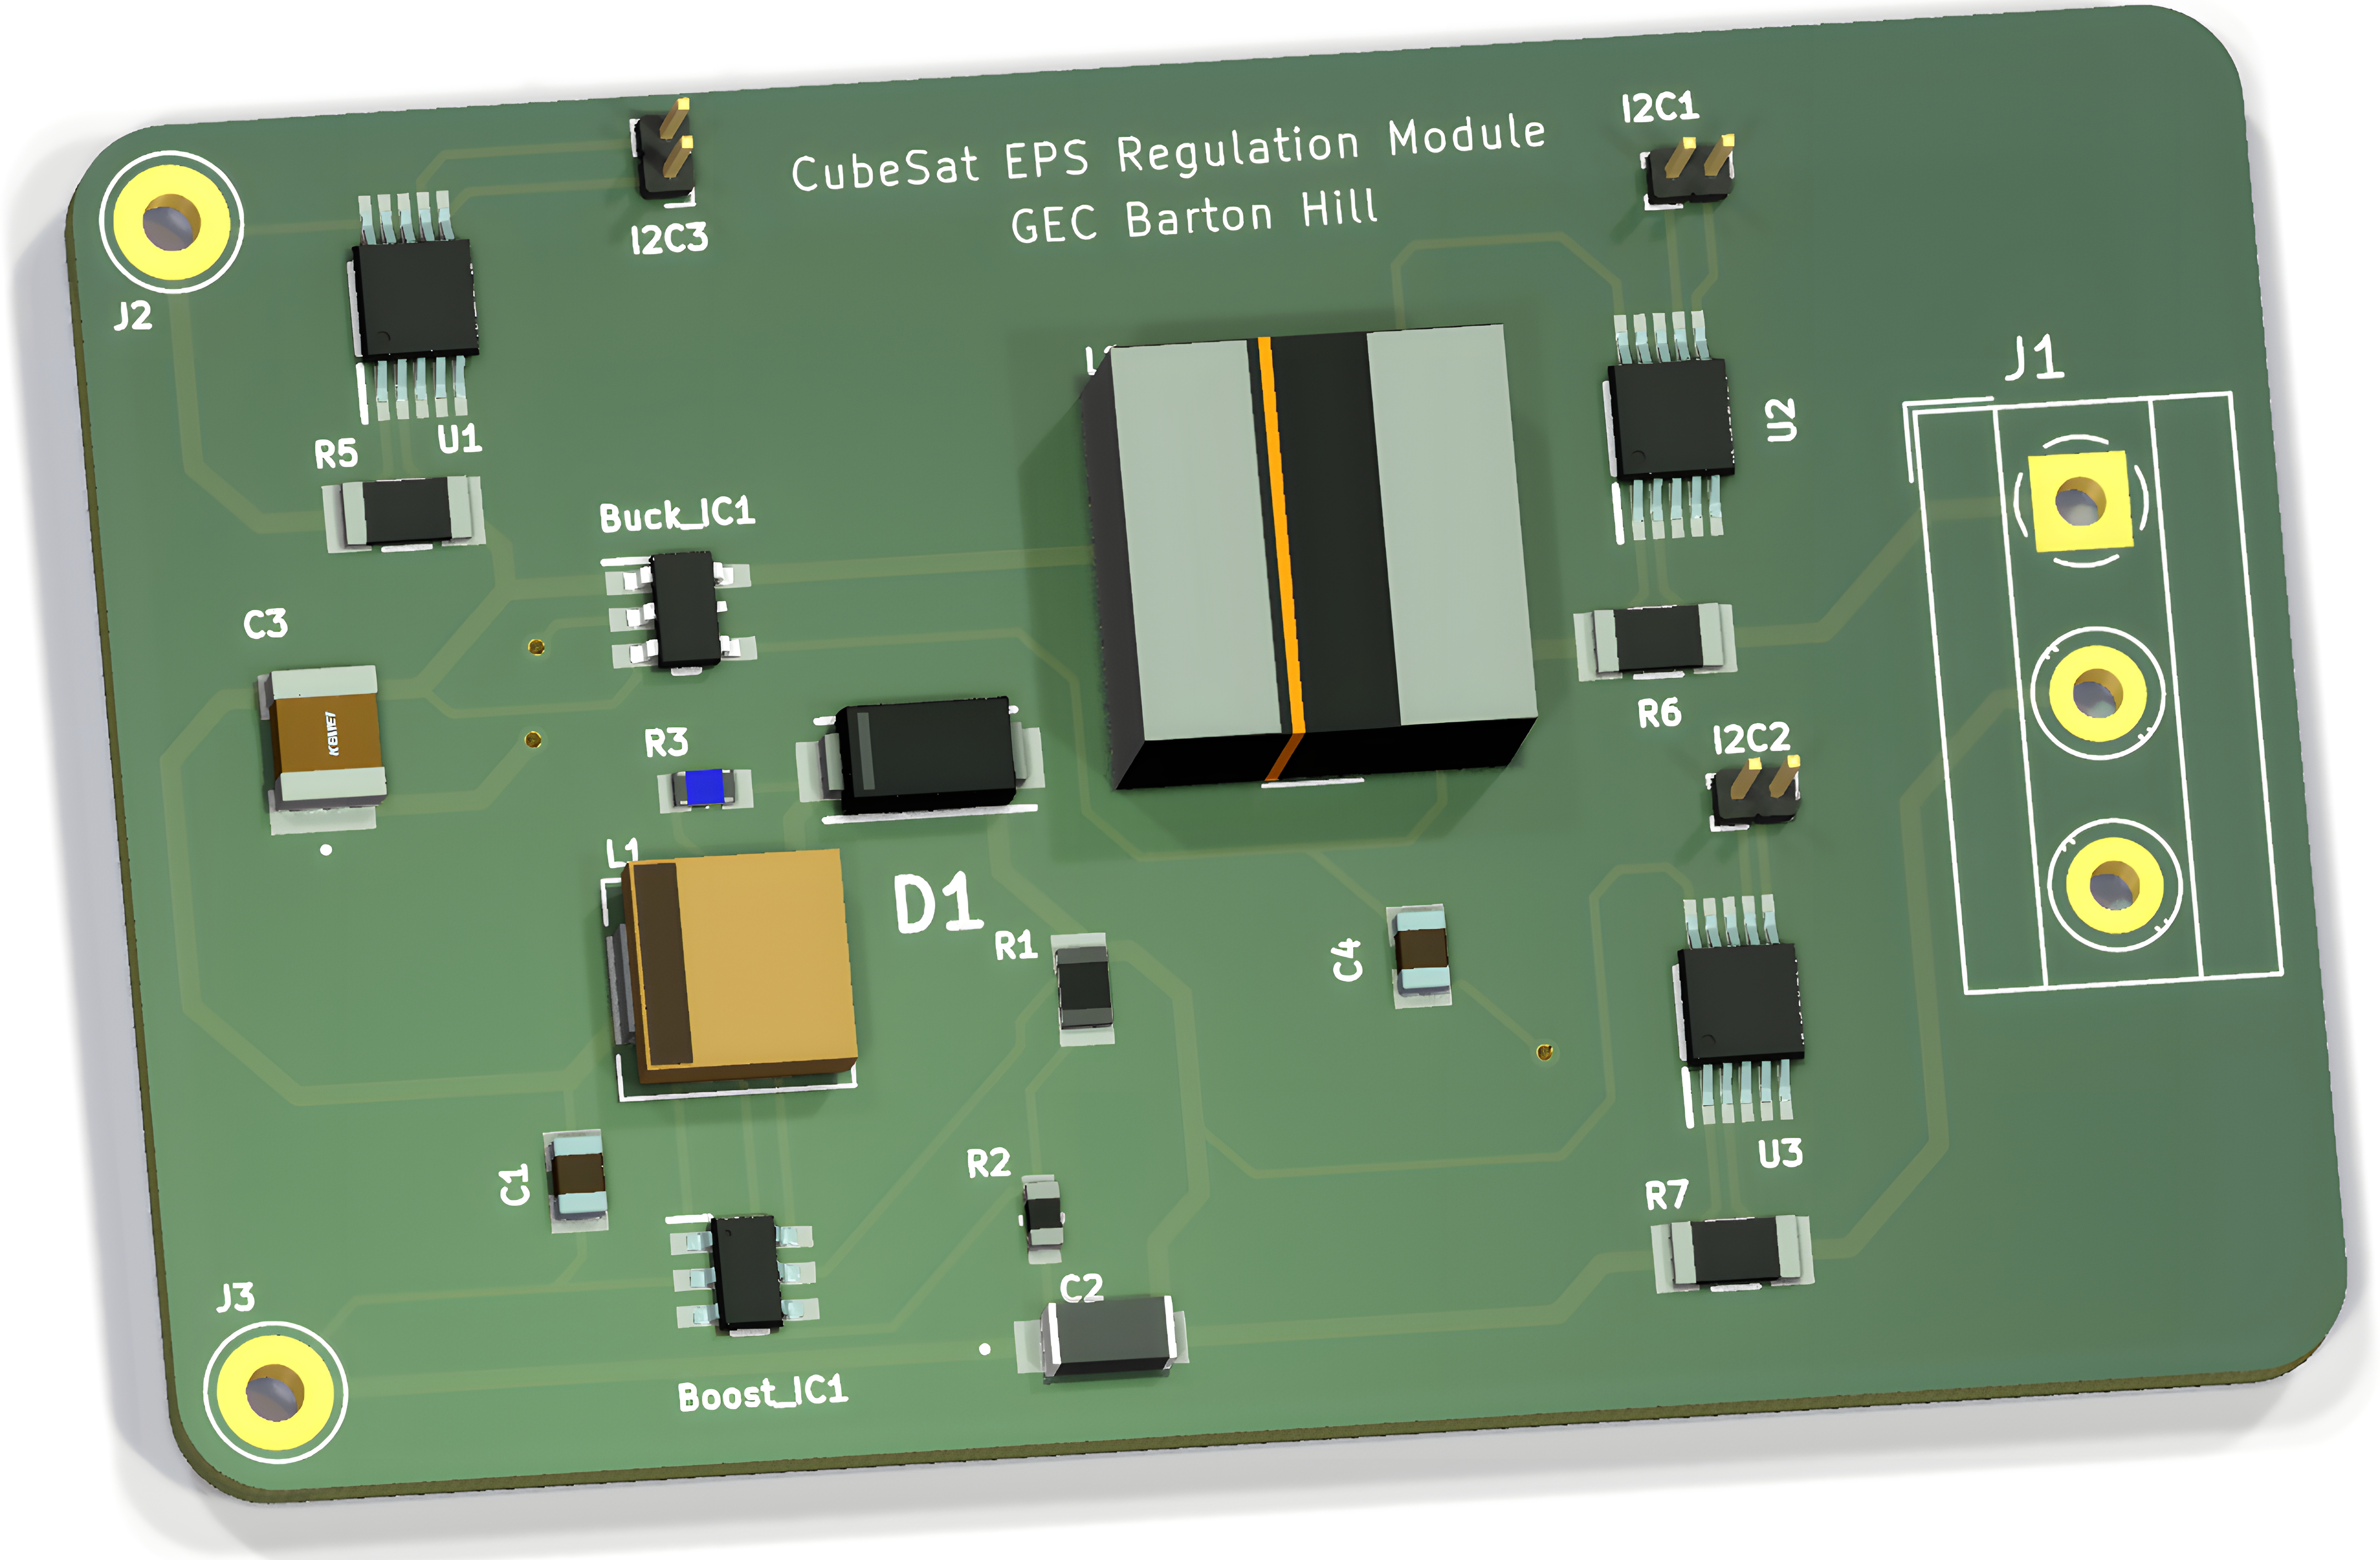
\includegraphics[width=0.6\columnwidth]{IMGS/1 3d.jpg}
 	\caption{\centering Buck and Boost circuit PCB - 3D Model}
 	\label{fig:bubopcb3d}
 \end{figure}
\pagebreak

 
 \section{Micro-controller}
 The requirements of micro-controllers depend of the BUS, the other links as digital/analog outputs, the energy consumption, the voltage range and the memory.
 \par
 The micro-controller has to handle the energy distribution of the entire CubeSat, and has to communicate with the OBC of CubeSat. Thus, it needs digital/analog outputs (for lines going to ADCS, Telemetry, OBC, battery , monitoring IC etc), UART for two-way communication between the micro-controller and the OBC and SPI to  send data of the battery level to the micro-controller.
 \par
 The micro-controller should have low energy consumption, around the mirco ampere range for the “Active mode” and around the hundreds of nano ampere for the “Off mode”. It also should need sufficient memory storage to store the readings to provide it to OBC when requested. It should also independently take action during over-current, over voltage happenings, and also should control different power modes of the EPS.
 \par
 Few considered options were Arduino, Raspberry Pi, TI micro-controllers, STM32 etc. Arduino has limited programming capabilities, and Raspberry Pi was too large for the need and also has high power consumption. STM32 was selected due to its wide range of capabilities, still maintaining the size and power constraints. It also has more community support which makes the programming easier.
 \par
 STM32 is a ARM Cortex M4 32-bit micro-controller having a flash memory of 512 Kb. It can have upto 81 I/O ports with interrupt capabilities. It can have upto 78 fast I/Os upto 42 MHz, 3 I2C interfaces, 3 USARTs, 4 SPIs etc. We selected STM32401RE development board to test its capabilities, and one of its advantage is that, it can be programmed using Arduino IDE or even MATLAB, apart from its own programming IDE called STM32CUBE IDE.

\pagebreak
\section{Component List}

% Please add the following required packages to your document preamble:
% \usepackage{graphicx}
\begin{table}[ht]
	\centering
	\resizebox{\textwidth}{!}{%
		\begin{tabular}{|llll|l|}
			\hline
			\multicolumn{1}{|l|}{\bf{Sl No.}} & \multicolumn{1}{l|}{\bf{Manufacturer Part\#}} & \multicolumn{1}{l|}{\bf{Description}} & \bf{Qty.} & \bf{Total + GST} \\ \hline
			\multicolumn{1}{|l|}{1} & \multicolumn{1}{l|}{C1210C475K4RACAUTO} & \multicolumn{1}{l|}{MLCC - SMD/SMT 16V   4.7uF X7R 1210 10\% AEC-Q200} & 4 & 287.4004211 \\ \hline
			\multicolumn{1}{|l|}{2} & \multicolumn{1}{l|}{CRCW0603510RJNEA} & \multicolumn{1}{l|}{Thick Film Resistors   - SMD 1/10watt 510ohms 5\%} & 10 & 38.62477875 \\ \hline
			\multicolumn{1}{|l|}{3} & \multicolumn{1}{l|}{C2012X7R1C105K125AA} & \multicolumn{1}{l|}{MLCC - SMD/SMT   1.0UF    16V   10\%          0805} & 4 & 78.42567444 \\ \hline
			\multicolumn{1}{|l|}{4} & \multicolumn{1}{l|}{SI3483DDV-T1-BE3} & \multicolumn{1}{l|}{MOSFET P-CHANNEL 30-V   (D-S)} & 3 & 175.6558838 \\ \hline
			\multicolumn{1}{|l|}{5} & \multicolumn{1}{l|}{CRA2512-FZ-R025ELF} & \multicolumn{1}{l|}{Current Sense   Resistors - SMD 0.025ohms 1\% +/- 50PPM} & 4 & 211.8081055 \\ \hline
			\multicolumn{1}{|l|}{6} & \multicolumn{1}{l|}{SRU1038-100Y} & \multicolumn{1}{l|}{Fixed Inductors 10uH   30\% SMD 1038} & 4 & 403.418396 \\ \hline
			\multicolumn{1}{|l|}{7} & \multicolumn{1}{l|}{ERA-1AEB102C} & \multicolumn{1}{l|}{Thin Film Resistors -   SMD 0201 1Kohm 0.1\% 25ppm} & 4 & 185.8752289 \\ \hline
			\multicolumn{1}{|l|}{8} & \multicolumn{1}{l|}{ERJ-PB6B3002V} & \multicolumn{1}{l|}{Thick Film Resistors   - SMD 0805 Anti-Surge Res. 0.1\%, 30Kohm} & 4 & 178.8937683 \\ \hline
			\multicolumn{1}{|l|}{9} & \multicolumn{1}{l|}{GRM21BR61C106KE15K} & \multicolumn{1}{l|}{MLCC - SMD/SMT 10uF   16Volts 10\%} & 10 & 136.0862885 \\ \hline
			\multicolumn{1}{|l|}{10} & \multicolumn{1}{l|}{ERJ-UP3F1303V} & \multicolumn{1}{l|}{Thick Film Resistors   - SMD 0603 Anti-sulfurated anti-surge resistor} & 4 & 100.4888077 \\ \hline
			\multicolumn{1}{|l|}{11} & \multicolumn{1}{l|}{IHLP2020CZER2R2M8A} & \multicolumn{1}{l|}{Power Inductors - SMD   2.2uH 6.6A 26Mohm} & 4 & 567.0136108 \\ \hline
			\multicolumn{1}{|l|}{12} & \multicolumn{1}{l|}{CL03A225KP3CRNC} & \multicolumn{1}{l|}{MLCC - SMD/SMT X5R,   2.2uF, +/-10\%, 10v, 0201} & 10 & 131.9122925 \\ \hline
			\multicolumn{1}{|l|}{13} & \multicolumn{1}{l|}{0805YC106KAT2A} & \multicolumn{1}{l|}{MLCC - SMD/SMT 16V   10uF X7R 0805 10\%} & 14 & 840.496582 \\ \hline
			\multicolumn{1}{|l|}{14} & \multicolumn{1}{l|}{GRM32ER71A226KE20L} & \multicolumn{1}{l|}{MLCC - SMD/SMT 1210   22uF 10volts X7R 10\%} & 4 & 309.7570496 \\ \hline
			\multicolumn{1}{|l|}{15} & \multicolumn{1}{l|}{WSHM2818R0600FEA} & \multicolumn{1}{l|}{Current Sense   Resistors - SMD .06ohms 7watt 1\%} & 4 & 478.3057251 \\ \hline
			\multicolumn{1}{|l|}{16} & \multicolumn{1}{l|}{CL10A106MP8NNNC} & \multicolumn{1}{l|}{MLCC - SMD/SMT   10uF+/-20\% 10V X5R 1 0603} & 10 & 74.97750854 \\ \hline
			\multicolumn{1}{|l|}{17} & \multicolumn{1}{l|}{SRN1060-100M} & \multicolumn{1}{l|}{Power Inductors - SMD   10uH 20\% SMD 1060} & 4 & 469.5845947 \\ \hline
			\multicolumn{1}{|l|}{18} & \multicolumn{1}{l|}{C2012C0G1H102J060AA} & \multicolumn{1}{l|}{MLCC - SMD/SMT   SUGGESTED ALTERNATE 810-C1005C0G1H102J} & 4 & 92.91137695 \\ \hline
			\multicolumn{1}{|l|}{19} & \multicolumn{1}{l|}{WSL2010R1100FEA} & \multicolumn{1}{l|}{Current Sense   Resistors - SMD 1/2watt .11ohms 1\%} & 4 & 295.6332397 \\ \hline
			\multicolumn{1}{|l|}{20} & \multicolumn{1}{l|}{C1005X8R1C473M050BB} & \multicolumn{1}{l|}{MLCC - SMD/SMT   RECOMMENDED ALT 810-C1005X8R1C473K0B} & 10 & 80.85810089 \\ \hline
			\multicolumn{1}{|l|}{21} & \multicolumn{1}{l|}{LTC3426ES6\#TRMPBF} & \multicolumn{1}{l|}{Switching Voltage   Regulators 1.2 MHz Step-Up DC/DC Converter} & 4 & 2723.537598 \\ \hline
			\multicolumn{1}{|l|}{22} & \multicolumn{1}{l|}{SMM4F5.0A-TR} & \multicolumn{1}{l|}{ESD Suppressors / TVS   Diodes 400W HI JCT TMP} & 2 & 132.8853455 \\ \hline
			\multicolumn{1}{|l|}{23} & \multicolumn{1}{l|}{SPV1040T} & \multicolumn{1}{l|}{Battery Management Hi   efficiency solar battery charger} & 4 & 2022.000854 \\ \hline
			\multicolumn{1}{|l|}{24} & \multicolumn{1}{l|}{CR0805-FX-9532ELF} & \multicolumn{1}{l|}{Thick Film Resistors   - SMD 95.3K 1\%} & 10 & 33.01148987 \\ \hline
			\multicolumn{1}{|l|}{25} & \multicolumn{1}{l|}{CMP2512-FX-3903ELF} & \multicolumn{1}{l|}{Thick Film Resistors   - SMD ResHighPower 2512 390k 1\% 1.5W TC100} & 4 & 243.4067993 \\ \hline
			\multicolumn{1}{|l|}{26} & \multicolumn{1}{l|}{ERJ-S02F2200X} & \multicolumn{1}{l|}{Thick Film Resistors   - SMD 0402 220ohms 1\% Anti-Sulfur} & 4 & 209.5628052 \\ \hline
			\multicolumn{1}{|l|}{27} & \multicolumn{1}{l|}{WSLP1206R0500FEA} & \multicolumn{1}{l|}{Current Sense   Resistors - SMD 1Watt 0.05Ohms 1\%} & 12 & 589.9055786 \\ \hline
			\multicolumn{1}{|l|}{28} & \multicolumn{1}{l|}{C3216JB1C226M160AB} & \multicolumn{1}{l|}{MLCC - SMD/SMT   RECOMMENDED ALT 810-C3216X5R1C226M} & 4 & 291.035675 \\ \hline
			\multicolumn{1}{|l|}{29} & \multicolumn{1}{l|}{RC0603FR-0730K9L} & \multicolumn{1}{l|}{Thick Film Resistors   - SMD 30.9 kOhms 100mW 0603 1\%} & 10 & 19.37921524 \\ \hline
			\multicolumn{1}{|l|}{30} & \multicolumn{1}{l|}{IHHP0805ZHER1R0M01} & \multicolumn{1}{l|}{Power Inductors - SMD   0805 1uH 20\%} & 4 & 216.9559174 \\ \hline
			\multicolumn{4}{|c|}{\bf{Total:}} & 11619.80762 \\ \hline
		\end{tabular}%
	}
\end{table}



\section{EPS PCB Design as per PC/104 Specifications}
  After all the selected components are tested separately and their proper working is ensured, these components can be combined together in a single PCB. This PCB is a four layer PCB with separate 3.3 and 5 V power planes and the bottom layer as the ground plane. A PC/104 connector is used for the ease of stackability of subsystems. As our aim is to design a 1U CubeSat, the PCB dimensions are limited to 9.5 cm x 9.5 cm. For simplifying the design process in KiCad, hierarchical sheets feature was used and the sheets were linked using global labels. The schematics of the different components in the EPS are shown below:

  \begin{figure}[h]
 	\centering
 	\includegraphics[width=0.99\columnwidth]{FrontMatter/pcb-MPPTv2.pdf}
 	\caption{\centering MPPT}
 	\label{fig:mpp 4lr}
 \end{figure}
 
   \begin{figure}[H]
 	\centering
 	\includegraphics[width=0.99\columnwidth]{FrontMatter/pcb-Battery Charger.pdf}
 	\caption{\centering Battery Charger}
 	\label{fig:batt 4lr}
 \end{figure}


  \begin{figure}[H]
 	\centering
 	\includegraphics[width=0.99\columnwidth]{FrontMatter/pcb-Regulation Module.pdf}
 	\caption{\centering Power Regulation circuits}
 	\label{fig:reg 4lr}
 \end{figure}
 
   \begin{figure}[H]
 	\centering
 	\includegraphics[width=0.99\columnwidth]{FrontMatter/pcb-ProtectionCircuit.pdf}
 	\caption{\centering Protection eFuse circuits}
 	\label{fig:protecc 4lr}
 \end{figure}

  \begin{figure}[H]
 	\centering
 	\includegraphics[width=0.99\columnwidth]{FrontMatter/pcb-MeasurementCircuit.pdf}
 	\caption{\centering Voltage and Current measurement circuits}
 	\label{fig:mes 4lr}
 \end{figure}
 
   \begin{figure}[H]
 	\centering
 	\includegraphics[width=0.99\columnwidth]{FrontMatter/pcb-STM32F405board.pdf}
 	\caption{\centering STM32 Micro-controller}
 	\label{fig:uC 4lr}
 \end{figure}


   \begin{figure}[H]
 	\centering
 	\includegraphics[width=0.99\columnwidth]{FrontMatter/pcb.pdf}
 	\caption{\centering PC/104 Connection Pins (Only pins connected to the EPS are labelled)}
 	\label{fig:pc104 4lr}
 \end{figure}
 
 
\section{3D Model}

 
 \begin{figure}[H]
 	\centering
 	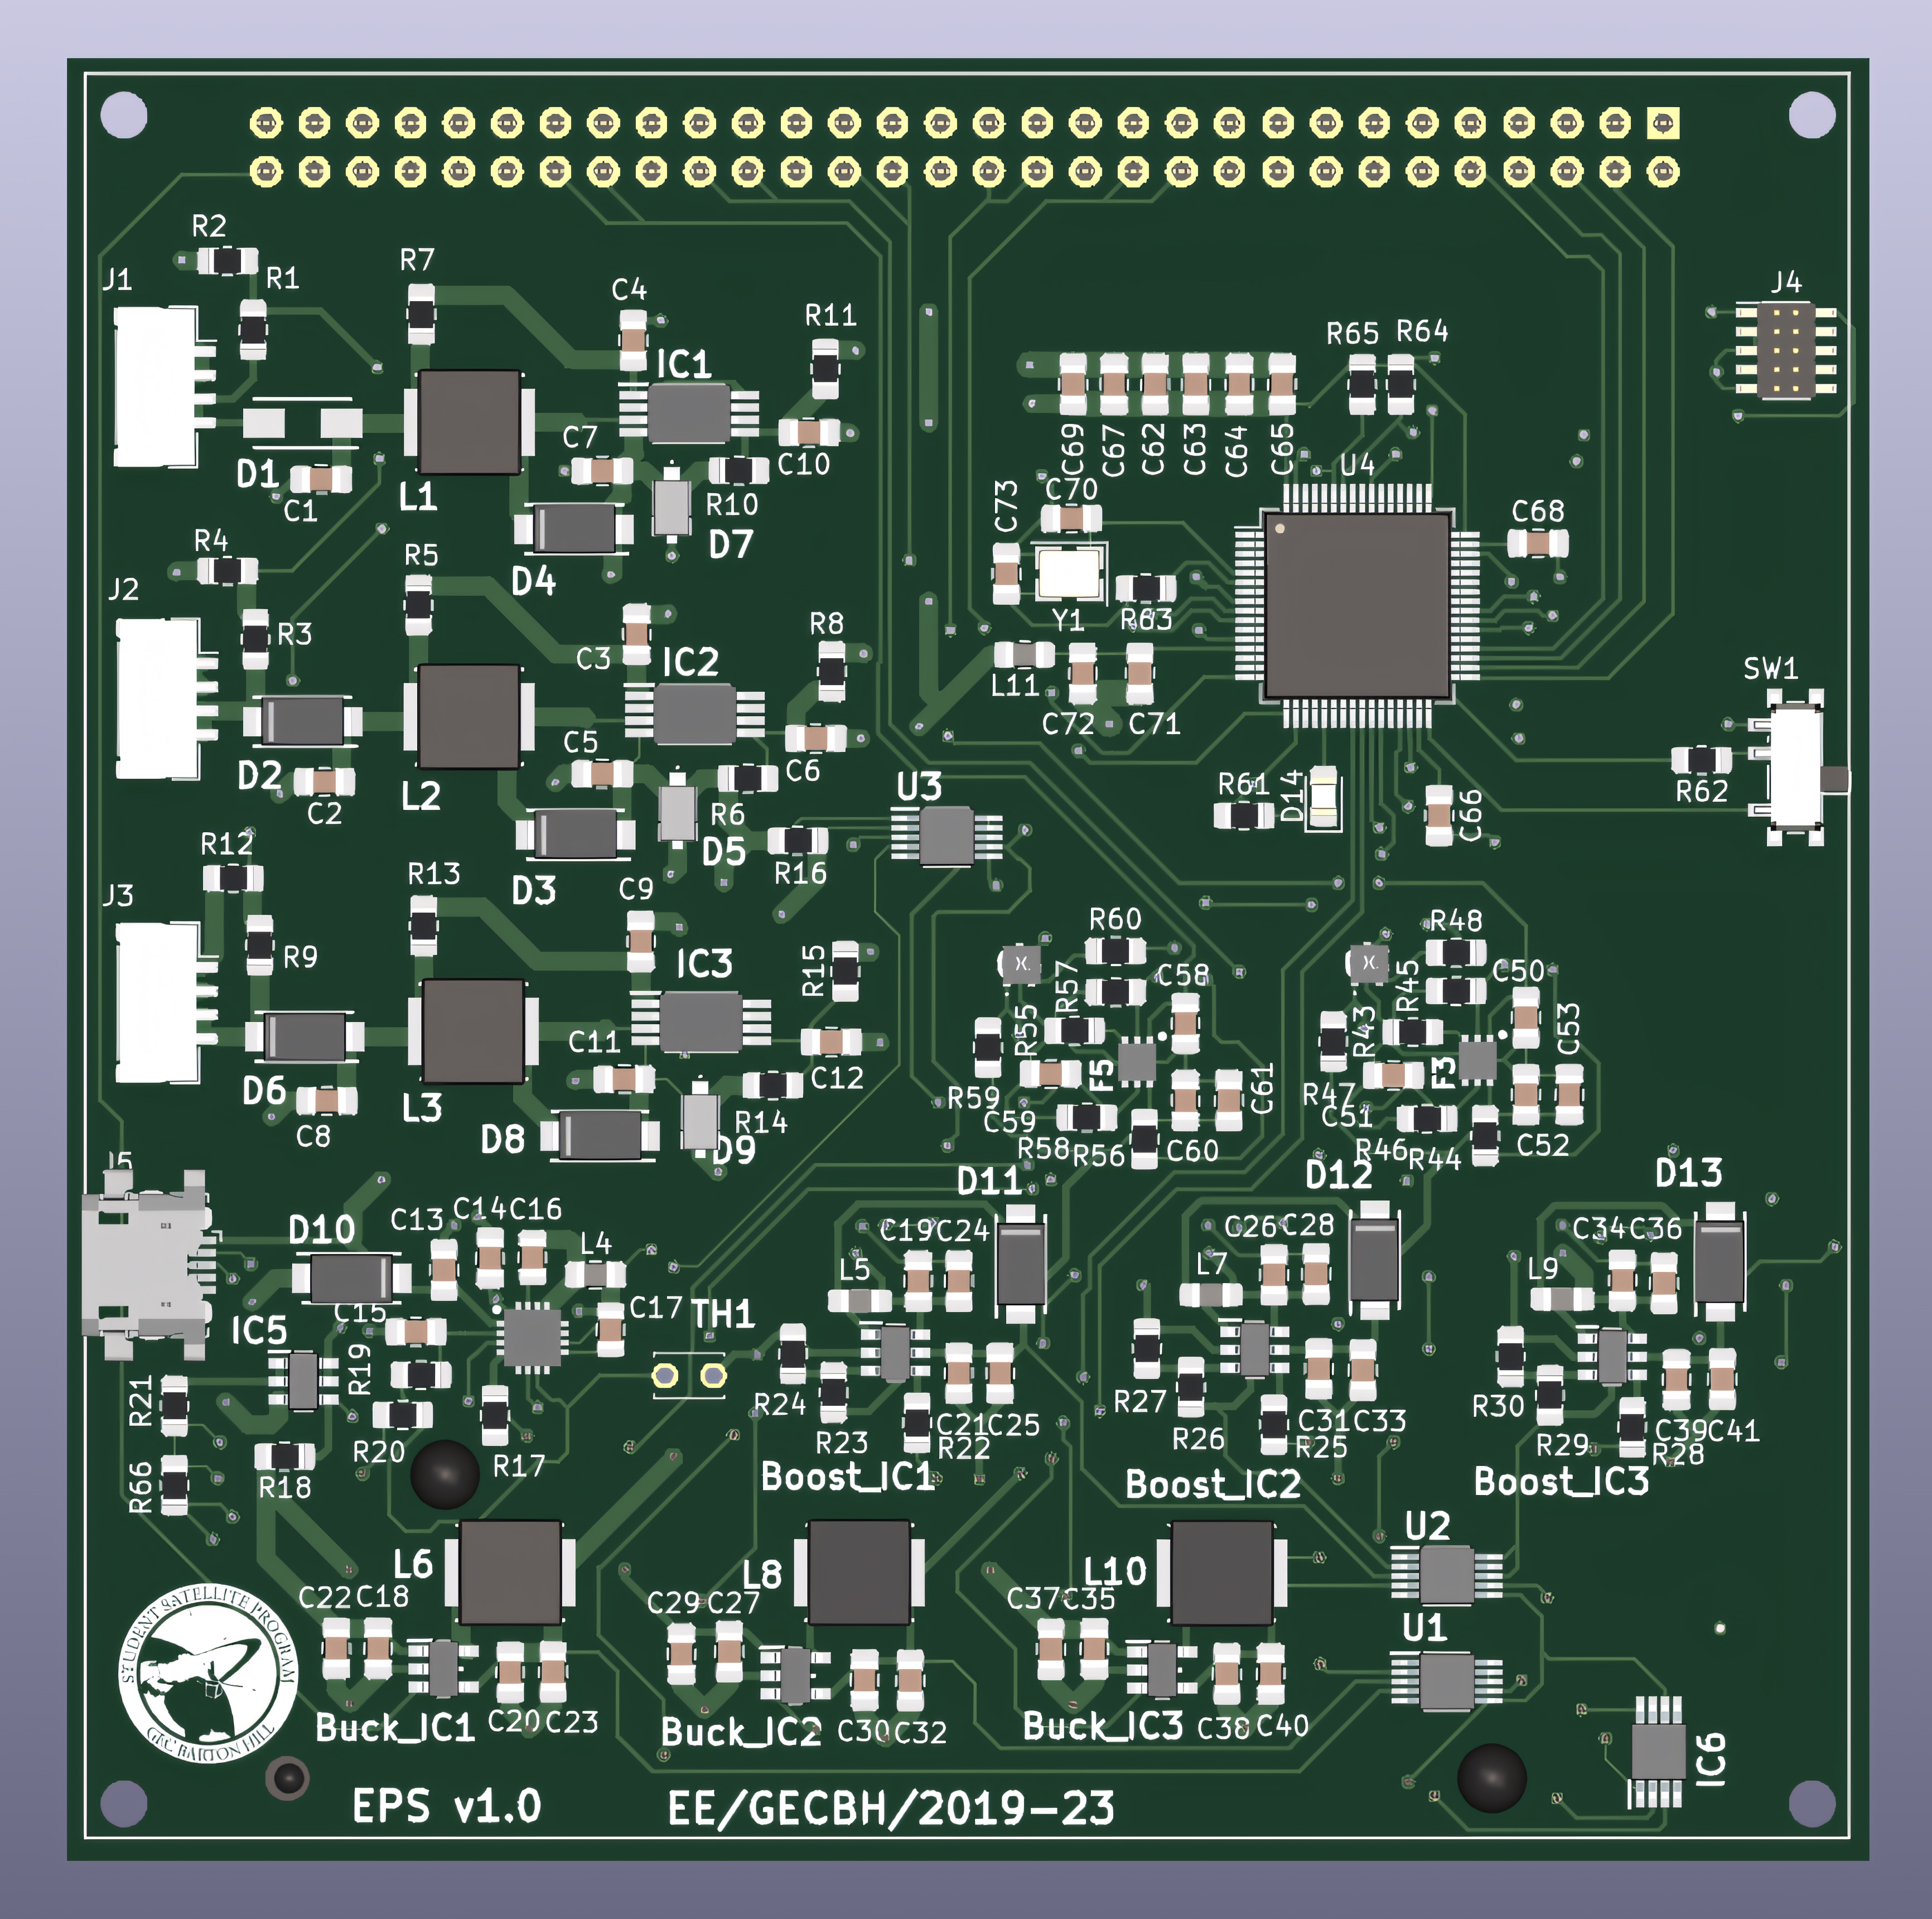
\includegraphics[width=0.99\columnwidth]{IMGS/eps_fr_4k.jpg}
 	\caption{\centering 3D Model of EPS PCB (Top Layer)}
 	\label{fig:eps3dfr}
 \end{figure}
 
 
  \begin{figure}[H]
 	\centering
 	\includegraphics[width=0.99\columnwidth]{IMGS/eps_bk-4k.jpg}
 	\caption{\centering 3D Model of EPS PCB (Bottom Layer)}
 	\label{fig:eps3dbk}
 \end{figure}
 
 
 %\pagebreak
 % \section{List of Components}
 % \begin{table}[h]
 % 	\begin{center}
 % 		\begin{tabular}{|l|l|l|}
 % 			\hline
 % 			{\bf Sl. No.} & {\bf Component} & {\bf Description} \\ \hline
 % 			1 & TPS62203 & Buck Converter IC \\ \hline
 % 			2 & LTC3426 & Boost Converter IC \\ \hline
 % 			3 & BQ25302 & Battery Charger IC \\ \hline
 % 			4 & Panasonic NCR 18650 GA & Battery \\ \hline
 % 			5 & SPV1040T & MPPT \\ \hline
 % 			6 & TJ Solar Cell 3G30C & Solar Cell \\ \hline
 % 			7 & STM 32 F401RE & Micro-controller \\ \hline
 % 			8 & Resistors &  \\ \hline
 % 			9 & Capacitors &  \\ \hline
 % 			10 & Inductors &  \\ \hline
 % 			11 & PCB &  \\ \hline
 % 		\end{tabular}
 % 		\caption{Components Required}
 % 		\label{table:3}
 % 	\end{center}
 % \end{table}